%!TEX TS-program = xelatex
%
% Created by Snow on 2017-11-14.
% Copyright (c) 2017 .
\documentclass{article}

\usepackage{polyglossia}
\usepackage{hyperref}
\usepackage{amsmath}
\usepackage{graphicx}
\usepackage[top=1in, bottom=1in, left=1.25in, right=1.25in]{geometry}


\newcommand{\projTitle}{SOME TITLE TO INSERT}

\title{COMP6111C Project Proposal}
\author{Authors}
\date{}

\begin{document}

\maketitle

\abstract{Abs...}

\section{Introduction}
The public cloud, such as Amazon EC2\cite{}, Microsoft Azure\cite{}, etc., has been an ideal place for users to host their applications in recent years. The cloud computing damatically benefit those users by providing low cost and pay-for-use computation resources, such as virtual machines (VMs). Users rent VMs from cloud service provider and deploy their applications inside VMs, such as web servers for HTTP request, FTP servers for file sharing and so on. With the increasing popularity of cloud computing, users begin to deploy some cretical applications or services, such as finacial analytical service or human resource management systems, on the cloud. How to gurantee that those services or applications will not fail acidently poses great challenges for both cloud providers and users. Traditionally, by deploying a monitoring and dignostic system, it can mitigate the risk of those grey failure, but we will show in the following parts that it is not easy and optimal for either the cloud provider or the users to deploy such an monitoring and dignostic systems.

\textbf{For cloud providers.}

\textbf{For users.}

\section{Proof-of-Statistics}
Proof-of-work has been identified as a major bottleneck of scalability of \textit{Bitcoin}  and has been tackled by replacing it with some useful work \cite{filecoin-storage} or with a new system architecture \cite{RSCoin-bank}.  Replacment of proof-of-work with some  
efficient actions in blockchain-based systems can bring a great number of benefits since the usually wasted resources aggreate to an enormous amount of  computational power \cite{bitcoin-comp-elec-power}. Cloud data centers are not an exception for such an 
improvement. Data center environements are usually highly optimized and any system resource wastage is considered as critical and intolerable \cite{google-ai-power, facebook-cold-storage-rack}. Due to such stringent data center requirements, in-data center services
shall not incur any overhead on the miners for maintaining a globally shared blockchain and shall not result in misuse of CPU or any other resource. Considering this, we propose a paradigm called 'Proof-of-Statistics', which employs the miners as ordinary computaion nodes
for performing statistical operations on received data. The CPUs and other resources are dedicated to actions that are extensively conducted in modern data centers \cite{microsoft-autopilot} and which provide the miners with a reward. 

\begin{figure}[h!]
  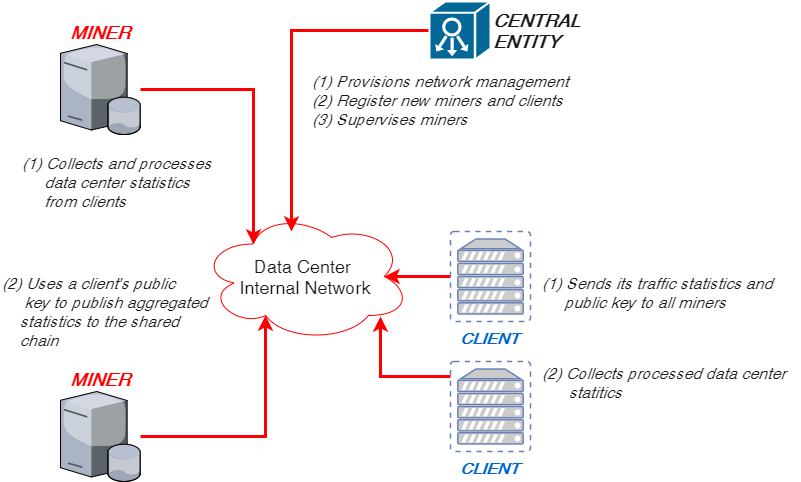
\includegraphics[width=0.6\linewidth]{figures/project_design.png}
  \caption{High-level Design of \textit{\projTitle}}
  \label{fig:project_design}
\end{figure}


\subsection{Data Flow and System Participants}
 \textit{Bitcoin} has applied a design of a globally shared ledger for recording all the transactions occured in the system \cite{bitcoin_paper}. Such a design introduces differentiation between system nodes: \textit{miners} and \textit{currency users}. As though, despite its architectural issues and perforamnce problems, \textit{Bitcoin} remains a global peer-to-peer network which is used by many users every day. Thus, it appears reasonable to adhere to the original proposal of \textit{Bitcoin} and segregate \textit{minders} from \textit{clients}. The proposed system, \textit{\projTitle}, exploits the fundamental principles of \textit{Bitcoin} with an extra entity: central controller, which, in data centers, may be the administrator of the data center (Figure \ref{fig:project_design}). The role of the central entity is minimal and is not crucial to implement the system. Though having a reliable controller unit simplifies the system and provides security benefits. The section will briefly explain the roles of each of the entities of the system and will describe a data processing path in the rest of the section.


\begin{figure}[h]
  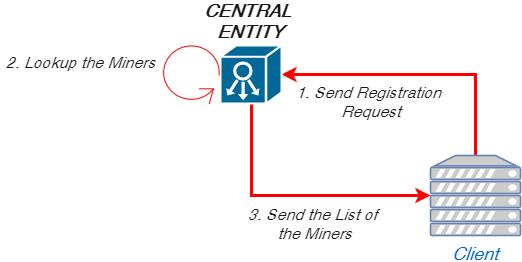
\includegraphics[width=0.5\linewidth]{figures/central_entity_client_reg.png}
  \caption{Central Entity-Client Interaction}
  \label{fig:central_entity_client_reg}
\end{figure}   

\paragraph{Central Entity (Controller):} The role of the central entity is more administrative than system-crucial. Many cloud data centers employ central control units for controlling system updates \cite{microsoft-autopilot}, data flows \cite{google_jupiter}, or system errors \cite{microsoft_netpoirot}. \textit{\projTitle} relies on a centralized controller for admitting new miners/clients to the system. Such an approach is chosen as currently most data centers do not support multicast packets and it is relatively expensive to flood a data center network in order to get approved as a new miner or a client. Hence, having a well-know service reduces system complexity and ensures that no data center bandwidth is wasted for just transmitting registration packets. The central entity accepts a new client and provides it with enough information about the current miners (miner IP addresses and their public encryption keyss) so that it can become a part of the global ecosystem (Figure \ref{fig:central_entity_client_reg}). After retrieving the needed information, the client directly interacts with miners to have its work processed and stored. Due to this, the involvement of the central entity is minimal and does not require any computationally-intensive opeartions for handling client requests. Scalability is considred in the design and should not be an issue as similar systems exist in real deployments \cite{hadoop_example}. The work assumes that a commodity server should suffice for running the service in most cloud data centers. 
\par


\noindent \newline On the other hand, the controller is also reponsible for approving new miners and supervising their integration into the current pool of miners. A new miner receives a list of the current miners $L$ and an approval certificate $Cr$ from the central entity.
The approval certificate $Cr$ is signed by the central entity to ensure other miners that the newcomer has been approved to be a miner \cite{public-auth-certificate}.

\paragraph{Clients:} Generating local system statistics (observing data flow latencies, thoughput, CPU utilization, and etc.) is prevalent in cloud data centers. However, the client of a data center can only be in charege of their own systems and are rather oblivious to the overall data center network. Despite storage of local system logs, measurements, the clients cannot go beyond their virtual networks (VNs) and are left with the locality drawback. Clients of \textit{\projTitle} can share their local statistics with the miners and get access to a more concise view of the entire network. A client is required to register for membership with the central entity (Figure \ref{fig:central_entity_client_reg}), and then directly communicate with the miners to send its local information about its system to the miners. The work assumes the clients are always honest and share their uncompromised information. However, if a client is dishonest and sends modified information to the miners, it may be identified as inconsistent and the client may lose its membership due to compromised statistics (\S\ \ref{ssec:work_of_miners}.     
\par       

\paragraph{Miners:} Collect various system metrics from clients and produce a concise summary for the clients in a form of a shared block-chain ledger. Miners are the core of the system and take similar reponsibilities to the ones in \textit{Bitcoin} (Figure \ref{fig:miner_work_flow}). The major responsibility of the miners is to process system metrics in a required manner. Miners define a set $O$ of operations that they are capable of applying on particular data from a set $M$. Clients must be aware of the sets and only
requests that comply with the both sets are processed by the miners. A request from a cloient is processed as it it described in (\S\ \ref{ssec:work_of_miners}) and the result of the request is shared among all the miners for voting and approval. Such a step is needed to
ensure that all miners have the same information and that 'lazy' miners would be identified and removed from the set of the current miners. The loss of membership in the current set of miners is not the major contribution of the work, so it is not described anu furhter except 
that a miner can lose its membership if other miners observe that the miner of interest is not contributing enough of its processing power. Each miner has to be aware of the other miners and keep track of a set $R_{miners} = \{r_1, ..., r_n\}$ which stores approximate rates, 
of  miners' result publishing. If a rate, $r_i$, goes below a mediate value, $m_{miner}$, of all rates in the set $R_{miners}$, miners vote for removing a particular miner $i$ from the current miners. If the vast majority of the miners agree on the removal of a miner $i$, 
the central entity must be informed about such a result so that the central entity would store the latest set of the current miners.    
\par


\begin{figure}[h]
  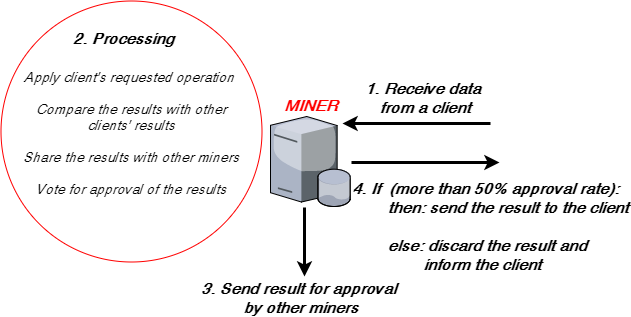
\includegraphics[width=0.5\linewidth]{figures/miner_work_diagram.png}
  \caption{Flow of a Miner's Work}
  \label{fig:miner_work_flow}
\end{figure}


\subsection{Work of Miners}\label{ssec:work_of_miners}


     
\newpage
\bibliographystyle{ieeetr}
\bibliography{proposal}

\end{document}

